% Options for packages loaded elsewhere
\PassOptionsToPackage{unicode}{hyperref}
\PassOptionsToPackage{hyphens}{url}
\documentclass[
  12pt]{article}
\usepackage{xcolor}
\usepackage{amsmath,amssymb}
\setcounter{secnumdepth}{-\maxdimen} % remove section numbering
\usepackage{iftex}
\ifPDFTeX
  \usepackage[T1]{fontenc}
  \usepackage[utf8]{inputenc}
  \usepackage{textcomp} % provide euro and other symbols
\else % if luatex or xetex
  \usepackage{unicode-math} % this also loads fontspec
  \defaultfontfeatures{Scale=MatchLowercase}
  \defaultfontfeatures[\rmfamily]{Ligatures=TeX,Scale=1}
\fi
\usepackage{lmodern}
\ifPDFTeX\else
  % xetex/luatex font selection
  \setmonofont[]{Menlo}
\fi
% Use upquote if available, for straight quotes in verbatim environments
\IfFileExists{upquote.sty}{\usepackage{upquote}}{}
\IfFileExists{microtype.sty}{% use microtype if available
  \usepackage[]{microtype}
  \UseMicrotypeSet[protrusion]{basicmath} % disable protrusion for tt fonts
}{}
\makeatletter
\@ifundefined{KOMAClassName}{% if non-KOMA class
  \IfFileExists{parskip.sty}{%
    \usepackage{parskip}
  }{% else
    \setlength{\parindent}{0pt}
    \setlength{\parskip}{6pt plus 2pt minus 1pt}}
}{% if KOMA class
  \KOMAoptions{parskip=half}}
\makeatother
\usepackage{longtable,booktabs,array}
\newcounter{none} % for unnumbered tables
\usepackage{calc} % for calculating minipage widths
% Correct order of tables after \paragraph or \subparagraph
\usepackage{etoolbox}
\makeatletter
\patchcmd\longtable{\par}{\if@noskipsec\mbox{}\fi\par}{}{}
\makeatother
% Allow footnotes in longtable head/foot
\IfFileExists{footnotehyper.sty}{\usepackage{footnotehyper}}{\usepackage{footnote}}
\makesavenoteenv{longtable}
\usepackage{graphicx}
\makeatletter
\newsavebox\pandoc@box
\newcommand*\pandocbounded[1]{% scales image to fit in text height/width
  \sbox\pandoc@box{#1}%
  \Gscale@div\@tempa{\textheight}{\dimexpr\ht\pandoc@box+\dp\pandoc@box\relax}%
  \Gscale@div\@tempb{\linewidth}{\wd\pandoc@box}%
  \ifdim\@tempb\p@<\@tempa\p@\let\@tempa\@tempb\fi% select the smaller of both
  \ifdim\@tempa\p@<\p@\scalebox{\@tempa}{\usebox\pandoc@box}%
  \else\usebox{\pandoc@box}%
  \fi%
}
% Set default figure placement to htbp
\def\fps@figure{htbp}
\makeatother
% definitions for citeproc citations
\NewDocumentCommand\citeproctext{}{}
\NewDocumentCommand\citeproc{mm}{%
  \begingroup\def\citeproctext{#2}\cite{#1}\endgroup}
\makeatletter
 % allow citations to break across lines
 \let\@cite@ofmt\@firstofone
 % avoid brackets around text for \cite:
 \def\@biblabel#1{}
 \def\@cite#1#2{{#1\if@tempswa , #2\fi}}
\makeatother
\newlength{\cslhangindent}
\setlength{\cslhangindent}{1.5em}
\newlength{\csllabelwidth}
\setlength{\csllabelwidth}{3em}
\newenvironment{CSLReferences}[2] % #1 hanging-indent, #2 entry-spacing
 {\begin{list}{}{%
  \setlength{\itemindent}{0pt}
  \setlength{\leftmargin}{0pt}
  \setlength{\parsep}{0pt}
  % turn on hanging indent if param 1 is 1
  \ifodd #1
   \setlength{\leftmargin}{\cslhangindent}
   \setlength{\itemindent}{-1\cslhangindent}
  \fi
  % set entry spacing
  \setlength{\itemsep}{#2\baselineskip}}}
 {\end{list}}
\usepackage{calc}
\newcommand{\CSLBlock}[1]{\hfill\break\parbox[t]{\linewidth}{\strut\ignorespaces#1\strut}}
\newcommand{\CSLLeftMargin}[1]{\parbox[t]{\csllabelwidth}{\strut#1\strut}}
\newcommand{\CSLRightInline}[1]{\parbox[t]{\linewidth - \csllabelwidth}{\strut#1\strut}}
\newcommand{\CSLIndent}[1]{\hspace{\cslhangindent}#1}
\setlength{\emergencystretch}{3em} % prevent overfull lines
\providecommand{\tightlist}{%
  \setlength{\itemsep}{0pt}\setlength{\parskip}{0pt}}
\usepackage{amssymb}
\usepackage{tikz}
\usetikzlibrary{positioning, arrows.meta, calc}
\usepackage[round]{natbib}
\usepackage{bookmark}
\IfFileExists{xurl.sty}{\usepackage{xurl}}{} % add URL line breaks if available
\urlstyle{same}
\hypersetup{
  pdftitle={Pre-Registration: Out of Touch: How Audience Reactions Shape Elite-Public Disconnect},
  pdfauthor={Sylvan Zheng},
  hidelinks,
  pdfcreator={LaTeX via pandoc}}

\title{Pre-Registration: Out of Touch: How Audience Reactions Shape
Elite-Public Disconnect}
\author{Sylvan Zheng}
\date{2026-02-23}

\begin{document}
\maketitle

\subsection{1. Introduction}\label{introduction}

The perception of disconnect between political and economic elites and
ordinary citizens is increasingly a concern for contemporary democratic
politics. Perceived disconnect is linked to declining institutional
trust, rising populist attitudes, and the erosion of shared epistemic
ground between citizens and governing institutions (Castanho Silva et
al. 2020; Guriev et al. 2023). Understanding how disconnect forms and
spreads is therefore central to understanding democratic backsliding,
institutional delegitimization, and the growing appeal of
anti-establishment politics.

The information environment and the Internet's influence on its
structure may play an important role in making disconnect visible. Under
traditional broadcast media, beliefs about how ordinary people are
faring were themselves largely formed from institutional sources, giving
rise to theories of sociotropic economic voting, epistemic authority,
and elite cueing (Kinder and Kiewiet 1981; {Zaller et al.} 1992;
Lewis-Beck and Stegmaier 2000). However, the Internet not only enables
the rapid spread of news, but also a dramatic rise in audience
reactions, commentary, and discussions of the news. Where institutional
sources once had near-monopoly control over public narratives about
economic conditions, audience comment sections now provide a visible
counter-signal at scale. This creates the conditions for systematic
visible divergence between what institutions report and what audiences
understand ordinary people to believe.

I focus on economic news and comments because institutional economic
reporting relies on aggregate indicators such as GDP growth,
unemployment rates, and inflation that track elite and investor welfare
more closely than median-household experience (Jacobs et al. 2021), and
may produce a persistent mismatch between official narratives and
citizens' lived reality. This is not hypothetical: from 2021 onward, the
U.S. experienced a striking divergence between macroeconomic indicators
and consumer sentiment (what commentators called the ``vibecession'').
GDP grew, unemployment fell to historic lows, and inflation eased from
its peak, yet consumer confidence remained persistently depressed
relative to fundamentals (Bolhuis et al. 2024). Comments on news
websites and social media filled with accounts of hardship, skepticism,
and frustration, illustrating the core dynamic: an institutional
narrative of recovery met by a visible popular counter-narrative of
continued struggle.

In this paper I develop a theory of perceived elite-public divergence in
which both the institutional economic signal and the popular commentary
signal --- independently and interactively --- shape perceived
disconnect and epistemic distrust. Positive economic news signals that
elites inhabit an informational world at odds with popular experience,
activating disconnect among readers who already perceive the economy
negatively. Negative reader comments signal that ordinary people are
struggling, shifting perceptions of popular economic experience and
making a public-elite gap visible even to those without strong economic
priors. When institutional and popular signals conflict, perceived
divergence between elite and popular accounts is maximized, predicting
effects on disconnect and epistemic distrust beyond what negative
information alone would generate. The experimental design tests two
distinct pathways: whether positive economic news directly activates
disconnect among economically dissatisfied readers, and whether negative
comments and positive news interact to create divergence effects.

\subsection{2. Relation to Existing
Literature}\label{relation-to-existing-literature}

\textbf{Democratic responsiveness and representation.} A growing
literature documents systematic failures of democratic responsiveness.
Legislators are more responsive to wealthy constituents and organized
interests than to the median voter (Bartels 2016) (Gilens 2012; Gilens
\& Page 2014), and Congressional staffers systematically misperceive
constituent opinion, overestimating conservatism due to disproportionate
contact with business interests (Hertel-Fernandez et al. 2019). These
failures matter: Castanho Silva et al. (2020) provide causal evidence
that perceived representation failures trigger populist attitudes,
particularly among those who did not previously hold them. The expansion
of mobile internet has compounded this dynamic by exposing citizens to
information about elite behavior that traditional media once filtered,
eroding government confidence and increasing populist vote shares
(Guriev et al. 2021). The mismatch condition in this study stages a
representation failure in miniature, making visible a gap between
institutional voices and popular experience.

\textbf{Economic news and the sentiment gap.} Since the pandemic,
consumer sentiment has been persistently depressed relative to
macroeconomic fundamentals, reflecting a disconnect between
institutional economic narratives and citizens' perceived reality
(Bolhuis et al. 2024). Economic news coverage contributes to this gap:
aggregate indicators like GDP and stock indices track top-income welfare
more closely than median-household welfare, giving economic reporting a
systematic class bias (Jacobs et al. 2021). Media framing of economic
conditions causally affects incumbent vote shares independent of actual
conditions (Garz and Martin 2021). Kowalski (2025) finds that citizens
across the political spectrum perceive a ``double disconnect'' between
economic data and lived experience, and between media discourse and
reality, fueling broad-based distrust in expertise not reducible to
partisanship.

\textbf{Populism, expertise, and epistemic trust.} Elite-public
disconnect is a core component of populist attitudes (Mudde 2004;
Akkerman et al. 2014; Schulz et al. 2018; Guriev et al. 2023). I study
three related outcomes: people-centered populism, perceived elite
unresponsiveness (Craig et al. 1990; Eulau and Karps 1977), and
epistemic distrust. Expertise's claims to objectivity are increasingly
contested, as expert prescriptions reflect professional socialization
and institutional interests as much as neutral knowledge (Dargent
Bocanegra and Lotta 2025). Bertsou and Caramani (2022) show that
technocratic and populist attitudes are distinct challenges to
representative democracy: technocrats prefer delegation to experts,
populists prefer popular sovereignty, and both express dissatisfaction
with existing arrangements. Mede and Schäfer (2020) extend this to the
epistemic domain with ``science-related populism,'' the view that
academic elites illegitimately claim sovereignty over ordinary people's
common sense. For economically strained respondents, the mismatch
condition erodes epistemic trust by confirming that institutional
knowledge sources serve elite rather than popular interests.

\textbf{The Internet and ``counter-elite'' information.} Under broadcast
media, economic narratives flowed from institutional sources to mass
audiences, giving elite information sources dominant influence on public
opinion (Kinder and Kiewiet 1981; {Zaller et al.} 1992; Druckman 2001).
The internet enables horizontal, peer-to-peer communication independent
of editorial control. This study shifts attention away from incivility
and polarization (Anderson et al. 2018; Thorson et al. 2010) to the
effect of audience-driven news discussion on second-order perceptions
and downstream effects on political attitudes (Cao, Xu, and Yang, 2026).
A broader implication is that authentic, but counter-elite information
(rather than misinformation) may be most potent in generating
institutional skepticism (as discussed by Allen et al. 2024 in the
context of the potent effects of true news about rare vaccine deaths on
vaccine hesitancy). This study applies similar logic to economic news:
negative comments are effective not because they expose people to
negativity but because authentic peer accounts of hardship, juxtaposed
against institutional reporting, make a gap between popular experience
and elite narrative visible --- a mechanism of source inference distinct
from the ``backfire effect'' (Nyhan and Reifler 2010), in which
corrections entrench misbeliefs through defensive motivated reasoning.

\subsection{3. Theoretical Framework}\label{theoretical-framework}

I propose that the information environment affects perceived elite
responsiveness, trust in media, and populist attitudes through perceived
elite-public divergence; that is, a disconnect between what news
audiences believe and what they think elites believe. When this
disconnect grows large, audiences feel that politicians are less
responsive, with less trust in epistemic institutions like the
mainstream media and expert opinion, and more supportive of populist
attitudes. Elite-public divergence arises from two distinct, but
potentially interacting features of the media environment:
institutionally backed news articles and reader reactions such as
comments on social media and news websites. For readers with strong
priors, conflicting news articles signal that elites are out of touch
with their reality, directly increasing disconnect. At the same time,
consensus from the ordinary public found in social media and news
comments that conflict with institutional narratives found in news could
demonstrate disconnect to a broader audience. This project tests these
two potent mechanisms in the context of economic news, where aggregate
institutional indicators frequently diverge from lived household
experience, a gap that has been both unusually wide and politically
salient in recent years.

The hypotheses below are organized around two outcome constructs.
Elite-public disconnect encompasses both people-centric populist
attitudes (the normative preference that ordinary people's will should
dominate politics) and perceived elite unresponsiveness (the belief that
officials do not act on public concerns). Although these dimensions are
conceptually distinct, they are predicted to co-move under the present
mechanisms and their combination yields better measurement reliability
than either sub-scale alone (see Appendix A). Epistemic distrust
(distrust in news media and expert institutions) is treated as a
separate primary outcome because it is a more direct consequence of the
divergence mechanism and less susceptible to alternative explanations
via general negativity; I expect epistemic distrust to therefore provide
the cleanest tests of the divergence mechanism.

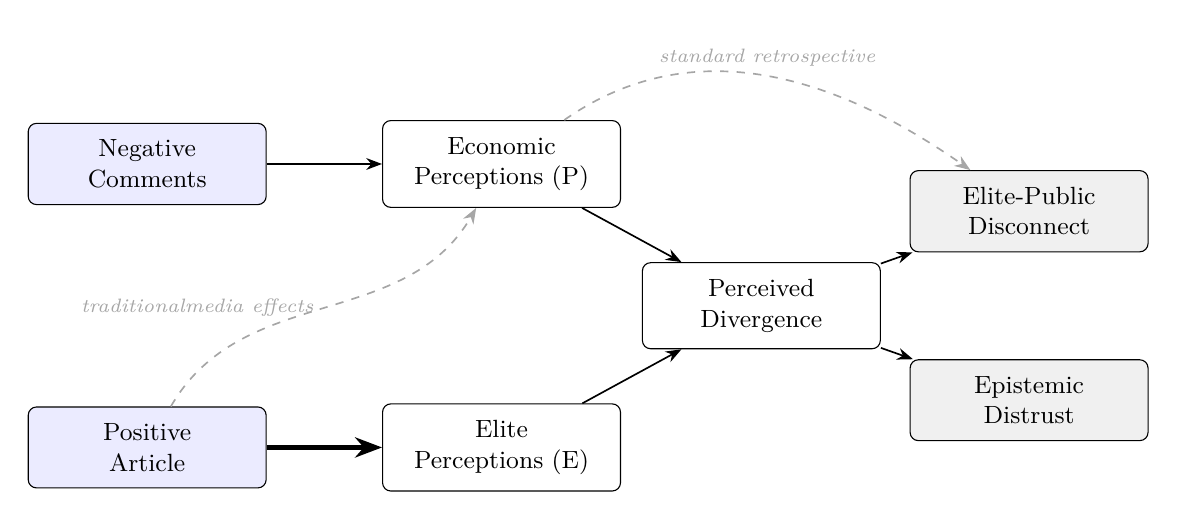
\begin{tikzpicture}[
  every node/.style = {font=\small},
  box/.style   = {draw, rounded corners=3pt, inner sep=6pt,
                  text width=2.6cm, align=center},
  treat/.style = {box, fill=blue!8},
  med/.style   = {box},
  res/.style   = {box, fill=gray!12},
  arr/.style   = {-Stealth, semithick},
  inst/.style  = {-Stealth, semithick, line width=1.5pt}
]

\node[treat] (cn)    at (0,    1.8)  {Negative\\Comments};
\node[treat] (ap)    at (0,   -1.8)  {Positive\\Article};
\node[med]   (econ)  at (4.5,  1.8)  {Economic\\Perceptions (P)};
\node[med]   (elite) at (4.5, -1.8)  {Elite\\Perceptions (E)};
\node[med]   (div)   at (7.8,  0)    {Perceived\\Divergence};
\node[res]   (disc)  at (11.2, 1.2)  {Elite-Public\\Disconnect};
\node[res]   (dist)  at (11.2,-1.2)  {Epistemic\\Distrust};

\draw[arr]  (cn)    -- (econ);
\draw[inst] (ap)    -- (elite);
\draw[arr]  (econ)  -- (div);
\draw[arr]  (elite) -- (div);
\draw[arr]  (div)   -- (disc);
\draw[arr]  (div)   -- (dist);

\draw[arr, dashed, gray!70] (econ)
  to[out=35, in=145]
  node[above, midway, font=\scriptsize\itshape] {standard retrospective}
  (disc);

\draw[arr, dashed, gray!70] (ap)
  to[out=60, in=240]
  node[left, midway, font=\scriptsize\itshape] {traditional\\media effects}
  (econ);

\end{tikzpicture}

According to conventional theory, positive economic news as an
authoritative, institutional signal should update readers' economic
views upward (Kinder and Kiewiet 1981; {Zaller et al.} 1992; Lewis-Beck
and Stegmaier 2000). However, I argue that for audiences with a baseline
strong negative perception of the economy, the opposite could occur. For
these readers, an upbeat news article signals that institutions (media,
analysts, experts) hold a view of the economy radically at odds with
their experience. While strained audiences may update their economic
perceptions upward in accordance with conventional theory, I argue that
exposure to positive economic news primarily shifts second order elite
economic beliefs; their beliefs about what elites believe about the
economy. A widening gap between readers' reality and what they believe
elites believe leads to disconnect outcomes: populism, perceived elite
unresponsiveness, and epistemic distrust.

Critically, the scope of implicated elites may extend beyond the news
source itself. Readers who encounter positive economic coverage may
impute similar views to politicians, public officials, and expert
institutions more broadly --- either because they believe these actors
rely on the same institutional media for economic information, or
through a more general process of trust transfer across elite groups
(Guo and Lei 2025). This dynamic is consistent with a wider literature
on the erosion of institutional credibility: as trust in media and
expert institutions has declined (Ladd 2012; Eyal 2019), positive
institutional signals may increasingly function as evidence of capture
rather than as useful information, activating skepticism across the
elite-institutional complex, not just toward the news outlet in
question.

\textbf{H1 (Article Backlash Effect)} Positive articles (compared to
negative articles) increase perceived elite-public disconnect (H1a) and
epistemic distrust (H1b) more for economically dissatisfied respondents.

\emph{Manipulation check.} Positive articles increase second-order
beliefs about the views of media elites, experts, and politicians.

\emph{Manipulation check.} Positive articles are trusted less by
economically dissatisfied respondents.

Comments also interact with news articles to affect disconnect
attitudes. Although the dominant framework in mass media and economic
voting research predicts that authoritative institutional sources should
crowd out anonymous ones, the authentic, unfiltered, nature of comments
means that readers can use them to make inferences about public opinion,
influencing reader's second-order beliefs about what ordinary people
think (Cao, Xu and Yang 2026). Negative comments that conflict with
positive economic news articles widen the perceived divergence between
perceptions of elite and public opinion about the economy, perhaps
regardless of economic priors.

This \emph{mismatch effect} means that negative comments in the context
of a positive article ought to increase disconnect perceptions. However,
negative comments could plausibly increase disconnect perceptions
through both the proposed divergence pathway and a ``standard
retrospective'' logic, where any negative economic information causes
audiences to be dissatisfied with elites directly. Therefore, the more
rigorous test compares the effect of negative comments between the
positive article context, where the divergence effect is expected, and a
negative article context, where no divergence effect is expected.

\textbf{H2 (Mismatch Effect).} The effect of negative comments on
perceived elite-public disconnect (H2a) and epistemic distrust (H2b) is
larger in the context of a positive article than a negative article.

Finally, I ask whether economically satisfied vs.~dissatisfied
respondents drive the mismatch effect. Priming effects would predict
that economically dissatisfied respondents are particularly activated in
the mismatch condition, producing the highest levels of perceived
disconnectedness compared to the economically satisfied. However, an
alternative account would suggest that if economically dissatisfied
respondents are already activated from the positive article alone (H1),
comments may not add much. Instead, the economically satisfied, who are
presented with actually new information about public economic attitudes
may be the ones who increase their disconnect perceptions most.

This research question has both interpretive and normative stakes. If
the dissatisfied are most affected, comments amplify existing
skepticism, helping explain the growing gap between consumer sentiment
and macroeconomic indicators, declining and polarizing media trust, and
the fracturing of shared epistemic reality along lines of economic
inequality. If the satisfied are most affected, comments expose readers
to perspectives they might not otherwise encounter, potentially serving
as a channel for bottom-up signaling that improves elite responsiveness
to public concerns.

\textbf{RQ1 (Mismatch Heterogeneity By Economic Satisfaction).} Is the
mismatch effect (defined as the H2 estimand) stronger or weaker for
economically dissatisfied audiences?

The table below maps the interpretive space across the primary result
combinations. H1 refers to the article-backlash hypothesis (positive
articles increase disconnect more for the economically dissatisfied); H2
refers to the mismatch hypothesis (negative comment effects larger in
the positive-article context). RQ1 sign indicates the direction of the
comment × econ\_pre interaction: + means economically satisfied
respondents show larger effects (learning); − means dissatisfied
respondents show larger effects (activation). Note that in the case that
H1 shows large effects, H2 effects are attenuated for the dissatisfied;
a null H2 could be masking a small comment-divergence effect for the
economically satisfied subgroup. A formal illustration of this can be
found in Appendix F.

\begin{tabular}{@{}cccp{11cm}@{}}
\hline
\textbf{H1} & \textbf{H2} & \textbf{RQ1} & \textbf{Interpretation} \\
\hline
$+$ & $+$ & + & Both channels. Article activates dissatisfied; comments provide divergence signal to satisfied. \\[3pt]
$+$ & $+$ & - & Both channels. Dissatisfied are activated by both article and comments; comments amplify existing grievance. \\[3pt]
$+$ & null & + & Dissatisfied saturated by article; satisfied show a small learning effect insufficient to break null aggregate H2. Weak support for comment-divergence channel. \\[3pt]
$+$ & Null & Null & Article-backlash channel only; comment-divergence effect below MDE. \\[3pt]
Null & $+$ & & Comment-divergence channel operating regardless of prior; RQ1 diagnostic of mechanism. \\[3pt]
Null & Null & & All effects below MDE. \\
\hline
\end{tabular}

\emph{Note on disconnect vs.~epistemic distrust.} Where the two outcomes
diverge, the pattern is diagnostic. Distrust effects without
corresponding disconnect effects favor the divergence mechanism
specifically --- institutional knowledge claims are implicated in a way
that a general negativity account would not predict.

\subsection{4. Design}\label{design}

\subsubsection{Experimental Conditions}\label{experimental-conditions}

2 (Article Tone: positive vs.~negative) × 2 (Comment Tone: negative
vs.~neutral) between-subjects factorial design.

{\def\LTcaptype{none} % do not increment counter
\begin{longtable}[]{@{}
  >{\raggedright\arraybackslash}p{(\linewidth - 4\tabcolsep) * \real{0.3333}}
  >{\raggedright\arraybackslash}p{(\linewidth - 4\tabcolsep) * \real{0.3333}}
  >{\raggedright\arraybackslash}p{(\linewidth - 4\tabcolsep) * \real{0.3333}}@{}}
\toprule\noalign{}
\begin{minipage}[b]{\linewidth}\raggedright
\end{minipage} & \begin{minipage}[b]{\linewidth}\raggedright
Neutral Comments
\end{minipage} & \begin{minipage}[b]{\linewidth}\raggedright
Negative Comments
\end{minipage} \\
\midrule\noalign{}
\endhead
\bottomrule\noalign{}
\endlastfoot
\textbf{Positive Article} & Elite-optimism signal only &
\textbf{Mismatch}: Elite-optimism and public-hardship signals diverge \\
\textbf{Negative Article} & Elite-pessimism signal only &
\textbf{Reinforcement}: Both signals indicate economic distress \\
\end{longtable}
}

\emph{Design Note: Neutral vs.~No Comments.} The control condition uses
neutral comments rather than a no-comments arm. A no-comments baseline
would cleanly isolate comment presence, but would confound tone with
text length, visual layout, and reading time --- all of which could
independently affect engagement and outcomes. Neutral comments hold
these structural features constant while varying only tone. The tradeoff
is ecological validity: purely neutral comment sections are uncommon
online, and a uniformly tepid section could signal curation or low
engagement. I accept this cost in exchange for cleaner identification of
tone effects. Pretesting (see Appendix D) confirms that neutral comments
are perceived as realistic in the article context.

\emph{Design Note: Unified vs.~Mixed Comment Tone.} All comments within
a condition share the same tone (all negative or all neutral) rather
than a realistic mix. Uniform tone maximizes treatment intensity --- if
the prior is that comment sections are heterogeneous and therefore
uninformative, a clear signal requires a strong dose. This is not wholly
unrealistic: comment threads often cluster in tone, as initial negative
reactions invite similar responses. Future designs could examine
dose-response effects using mixed-tone conditions.

\subsubsection{Stimuli}\label{stimuli}

\textbf{Articles:} Participants are randomly assigned to one of two
article stimuli per article-tone condition, following Fong and Grimmer
(2023). Two positive articles report favorable economic indicators
attributed to a mainstream news outlet; two negative articles report
unfavorable indicators. One article in each pair takes a general
economic conditions framing; the other focuses on job growth. The
positive jobs-focused article is adapted from real news reporting on the
January 2026 Bureau of Labor Statistics nonfarm payroll release, in
which job growth substantially exceeded expectations and the
unemployment rate fell below consensus forecasts. Both positive and
negative articles were pre-tested for perceived realism, perceived tone,
and first-order manipulation effectiveness; results are reported in
Appendix D.

\textbf{Comments:} Below the article, participants will see 4 user
comments (either all negative or all neutral). Negative comments express
economic hardship. Neutral comments offer factual observations or
balanced reactions. Comment order is randomized across participants.
Each comment is displayed with a randomly assigned like count (range
1--15) to increase ecological realism; participants are randomly
assigned to a low (1--10) or high (6--15) engagement condition, ensuring
coverage of both ends of the range. Like counts are recorded as embedded
data to facilitate exploratory analysis of engagement cues. Comments
were pre-tested for perceived tone and realism; results are reported in
Appendix D.

\subsubsection{Sample}\label{sample}

\textbf{N = 2,400} recruited via Prolific, yielding approximately 600
per cell.

\textbf{Quota-Sampling and Block Randomization}

I plan to quota sample to meet even third distribution on party ID
(Democrat/Independent/Republican) and even split on college degree
vs.~no college degree.

This design corrects Prolific's approximately 60--70\% college-educated
and Democrat skew. Equal representation on education and party ID is
important as both are heavily correlated with populism attitudes and
economic perceptions. Income was considered as a potential secondary
quota variable but dropped because of operational complexity and because
income and education are already correlated.

Participants will further be block-randomized based on their responses
to the economic perceptions question (econ\_pre). This helps maximize
power for the most theoretically interesting heterogeneous effects
analysis.

\subsubsection{Procedure}\label{procedure}

\begin{enumerate}
\def\labelenumi{\arabic{enumi}.}
\tightlist
\item
  Informed consent
\item
  Pre-treatment measures: econ\_pre, econ\_identity, 5 political
  attitude items (see Section 5), news interest, party identification.
\item
  Treatment exposure: article + negative or neutral comments
\item
  Post-treatment outcomes: full outcome battery, economic perceptions,
  media trust, article trust, comment credibility, attention check,
  manipulation check
\item
  Auxiliary demographics are provided by Prolific data
\end{enumerate}

\textbf{Exclusion criteria.} Respondents are excluded if they: (a) fail
the post-treatment attention check or (b) complete the survey in under
180 seconds. Exclusions are applied before all analyses; excluded
respondents are described in Appendix C.

The 180-second cutoff is set at approximately half the median completion
time in Pilot 3 (median: 6:30), targeting only egregious cases. In Pilot
3, 4 of 248 respondents failed the attention check and 4 met the speeder
threshold (one of whom also failed an attention check), yielding 7
unique exclusions. This conservative approach is consistent with
Greszki, Meyer, and Schoen (2015), who find that removing speeders
rarely improves data quality.

\subsection{5. Measures}\label{measures}

\subsubsection{Pre-Treatment}\label{pre-treatment}

\begin{itemize}
\tightlist
\item
  \textbf{National economic perceptions (econ\_pre; primary moderator):}
  ``Over the past year, would you say that the national economy has
  gotten better, stayed about the same, or gotten worse?'' (5-point:
  Much Better to Much Worse). The activation and learning mechanisms
  require a prior about how the economy is faring; econ\_pre captures
  this directly and has stronger theoretical grounding for the
  divergence mechanism than reference-group perceptions. Pilot studies
  use econ\_pre throughout.
\item
  \textbf{Economic identity (econ\_identity; robustness moderator):}
  ``Now thinking not of yourself personally, but thinking of people like
  you --- how do you think people like you are doing financially right
  now?'' (5-point: Much worse to Much better; adapted from Nagler et al.
  (2022)). Captures reference-group economic perceptions; less
  susceptible to partisan expression than econ\_pre but measures a
  somewhat different construct. All het effects analyses are replicated
  with econ\_identity as a robustness check. If the two moderators
  diverge substantially (r \textless{} 0.4), both are reported and
  differences noted.
\item
  \textbf{Pre-treatment political attitudes (5 items; controls):} A
  battery of items related to the main outcome items, administered
  before treatment to absorb baseline variation without repeating
  outcome measures: ``Politicians need to follow the will of the
  people''; ``The system is stacked against people like me''; ``Public
  officials care about what people like me think'' (rev); ``The news
  media presents fair and accurate information'' (rev); ``When it comes
  to public policy, I'd rather put my trust in experts than the opinions
  of ordinary people'' (rev). (Variables: pop\_pre2--pop\_pre6.)
\item
  \textbf{News interest:} ``How much attention do you pay to news about
  public affairs?'' (4-point)
\item
  \textbf{Party identification:} 3-category (Democrat / Independent /
  Republican)
\end{itemize}

\emph{Note on pre-treatment item selection.} The five political attitude
items were initially organized as 2 items per outcome dimension
(people-centrism; elite responsiveness; epistemic distrust), providing a
pre-treatment analog for each scale without fully replicating the
post-treatment battery. In Pilot 3, this set achieves R² \(\approx\) 0.6
for both outcome indices, confirming meaningful variance absorption.
Personality items (Big 5; pers1, pers2) were tested but dropped due to
near-zero marginal R² contribution across all outcomes. Pilot 3 also
showed that ``Politicians need to listen closely to the problems of the
people'' showed no additional \(R^2\) gain over the simpler
``Politicians need to follow the will of the people'' (the classic
populism measure used in Akkerman et al. (2014)), so this item will also
be dropped, leaving five total items. Appendix E shows the marginal
\(R^2\) gain per covariate.

\subsubsection{Post-Treatment Outcomes}\label{post-treatment-outcomes}

The first primary outcome combines survey items measuring people-centric
populism attitudes and attitudes toward elite responsiveness into a
single \textbf{Elite-Public Disconnect} index (6 items). The populism
items draw on established populism scales (Akkerman et al. 2014; Schulz
et al. 2018; Castanho Silva et al. 2020) and capture the normative
preference that ordinary people's will ought to be the dominant
consideration in politics. The elite responsiveness items build on the
external political efficacy tradition, anchored by the ANES item on
whether public officials care about ordinary people (Campbell et al.
1954; Craig et al. 1990), and extend this by including items from
American populism research on anti-system attitudes (Oliver and Rahn
2016) and a specific measure of perceived politician understanding of
the respondent's economic reality used by the SSRS Economic Attitudes
Tracker. In pilot data, the 6 disconnect items have strong inter-item
reliability (\(\alpha = 0.73\)).

The second primary outcome \textbf{Epistemic distrust} captures trust in
knowledge institutions --- experts and news media --- and connects to
the science-related populism and media trust literatures (Mede and
Schäfer 2020; Ladd 2012). All scales are coded so that higher values
indicate greater disconnect/distrust. In pilot data, the 3 epistemic
distrust items have inter-item reliability \(\alpha = 0.65\). This falls
below the conventional 0.70 threshold, but the scale is not designed to
be internally homogeneous: trust in experts and trust in news media are
theoretically distinct dimensions that need not co-move, and the low
alpha reflects this rather than measurement error. The index is
justified on content validity grounds.

\textbf{Index construction.} Each index is formed as a simple unweighted
additive average of its component items (after reverse-coding where
indicated), then standardized to mean 0, SD 1 using the full
post-exclusion sample. Full-sample standardization is used rather than
control-group standardization because the 2×2 design has no pure control
cell --- every respondent is exposed to an article and comments ---
making a single reference cell an arbitrary choice. Standardizing to the
full sample yields effect sizes in SD units of the experimental
distribution and ensures comparability across outcomes and hypotheses.
Raw-scale analyses are reported as a robustness check. Individual item
results will also be reported in supplementary analyses.

Appendix A provides further details on scale structure including results
of a supporting exploratory factor analysis based on pilot data.

\begin{enumerate}
\def\labelenumi{\arabic{enumi}.}
\tightlist
\item
  \textbf{Elite-Public Disconnect} (6-item index; higher = more
  disconnected):

  \begin{itemize}
  \tightlist
  \item
    ``Politicians ought to be following the will of the people''
    (will\_of\_ppl; Akkerman et al. (2014); Bertsou and Caramani (2022))
  \item
    ``It's important for a political leader to be like the people he or
    she represents'' (leader\_represent; Castanho Silva et al. (2020);
    Bertsou and Caramani (2022))
  \item
    ``Politics is a fight between the good people and the corrupt
    elite'' (good\_corrupt; Akkerman et al. (2014))
  \item
    ``Public officials care about what people like me think'' (rev;
    higher values coded as less perceived responsiveness;
    public\_officials\_rev; ANES, Campbell et al. (1954))
  \item
    ``Politicians understand the economic reality I am living in'' (rev;
    econ\_reality\_rev; SSRS Economic Attitudes Tracker)
  \item
    ``The system is stacked against people like me'' (system\_stacked;
    Oliver and Rahn (2016))
  \end{itemize}
\item
  \textbf{Epistemic Distrust} (3-item index; higher = less trust):

  \begin{itemize}
  \tightlist
  \item
    ``When it comes to public policy, I'd rather place my trust in
    experts than the opinions of ordinary people'' (rev;
    trust\_experts\_rev; Oliver and Rahn (2016); Bertsou and Caramani
    (2022))
  \item
    ``Experts often claim to know what's best, but they're frequently
    out of touch with reality'' (experts\_claim; new item)
  \item
    ``How much, if any, would you say you trust the information you get
    from national news organizations?'' (rev; news\_trust\_rev; ANES)
  \end{itemize}
\item
  \textbf{Economic Perceptions (econ\_post):}

  \begin{itemize}
  \tightlist
  \item
    Same item as econ\_pre, post-treatment.
  \end{itemize}
\item
  \textbf{Second-Order Economic Perceptions:}

  \begin{itemize}
  \tightlist
  \item
    ``How well do you think a typical {[}member of the media / economic
    expert / politician / citizen{]} thinks the economy is doing?''
    (so\_media, so\_expert, so\_politician, so\_citizen; 5-point scale,
    same anchors as econ\_pre). Elite-perception and public second-order
    beliefs; manipulation check for effects on perceived elite economic
    views.
  \end{itemize}
\end{enumerate}

\subsubsection{Other Demographics}\label{other-demographics}

I plan to collect the following demographic information about
respondents automatically via Prolific.

\begin{itemize}
\tightlist
\item
  Age, gender, race/ethnicity, education, income, perceived SES,
  employment status
\end{itemize}

\subsection{6. Analysis Plan and Pilot
Results}\label{analysis-plan-and-pilot-results}

Throughout this section, I illustrate the analysis strategy using data
from a pilot study (N \(\approx\) 240). Details of the pilot sample are
reported in Appendix C.

All models estimated with OLS. Robust standard errors reported
throughout.

\textbf{Multiple comparisons.} I do not apply family-wise correction
across outcomes. Each hypothesis is an individual test of a
theoretically distinct claim at \(\alpha = 0.05\): a world in which only
H1a holds is genuinely different from one in which only H2a holds, and
both are independently informative. Alpha adjustment is warranted only
under disjunction testing --- where at least one significant result is
required to reject a joint null --- which does not describe my
hypothesis structure (Rubin 2021). Exploratory analyses are reported
descriptively without inferential claims.

\textbf{Specification 1 (Pre-registered controls):} All models include
\(\delta X_i\), where \(X_i\) includes: econ\_identity, econ\_pre,
pre-treatment disconnect items, party ID, news interest, education, and
income.

\textbf{Specification 2 (Saturated controls):} Adds age, gender,
race/ethnicity, employment status, and perceived SES to the
Specification 1 covariate set. Results are not expected to differ
materially given the strong pre-treatment adjustment in Specification 1.

\textbf{Specification 3 (Unadjusted):} No covariates. Reported as a
tertiary robustness check to confirm results are not an artifact of
covariate selection.

\subsubsection{Manipulation Check: Second-Order
Beliefs}\label{manipulation-check-second-order-beliefs}

The article manipulation should shift respondents' second-order beliefs
about elite economic views (so\_media, so\_expert, so\_politician); this
is the first-stage check for the H1 channel. Estimated across the full
2×2 sample:

\[Y_i = \beta_0 + \beta_1 \text{AP}_i + \beta_2 \text{CN}_i + \beta_3 \text{AP}_i \times \text{CN}_i + \delta X_i + \epsilon_i\]

\begin{figure}
\centering
\pandocbounded{
\includegraphics[keepaspectratio,alt={Effects of treatment conditions on post-treatment economic perceptions and second-order beliefs. OLS coefficients with 95\% CIs; pre-registered controls. Pilot 3 attention-passing sample, all four arms (N = 240).}]{figures/manip.so.pilot4.png}}
\caption{Effects of treatment conditions on post-treatment economic
perceptions and second-order beliefs. OLS coefficients with 95\% CIs;
pre-registered controls. Pilot 3 attention-passing sample, all four arms
(N = 240).}
\end{figure}

\emph{Pilot results.} The positive article shifts second-order beliefs
about media, experts, and politicians by nearly a full scale point --- a
large effect for a brief news exposure --- and this shift is consistent
across comment conditions (interaction near zero). Negative comments
show a marginally significant effect on perceived citizen economic
conditions (so\_citizen) and overall economic outlook, but this effect
is concentrated in the negative-article arm; in the positive-article
arm, article and comment effects on these measures largely cancel.

\subsubsection{H1: Article Backlash (H1a,
H1b)}\label{h1-article-backlash-h1a-h1b}

Estimated within the \textbf{neutral comments arm} (N \(\approx\)
1,200), where no competing comment signal is present:

\[Y_i = \beta_0 + \beta_1 \text{AP}_i + \beta_2 \text{EP}_i + \beta_3 \text{AP}_i \times \text{EP}_i + \delta X_i + \epsilon_i\]

where EP = econ\_pre. The coefficient of interest is \(\beta_3\).
\textbf{H1a} predicts \(\beta_3 < 0\) for disconnect: positive articles
increase disconnect more for economically dissatisfied respondents.
\textbf{H1b} predicts \(\beta_3 < 0\) for epistemic distrust. I report
marginal effects of article\_positive across the econ\_pre distribution
(1--5) for both outcomes. The full 2×2 sample controlling for comment
condition is reported as a robustness check; econ\_identity substituted
for econ\_pre is a second robustness check.

\begin{figure}
\centering
\pandocbounded{
\includegraphics[keepaspectratio,alt={Marginal effects of positive articles by pre-treatment economic perceptions (econ\_pre). Neutral-comments arm (N \textbackslash approx 60), Specification 1 controls. Shaded bands are 95\% CIs. Pilot 3.}]{figures/article.main.het.pilot4.png}}
\caption{Marginal effects of positive articles by pre-treatment economic
perceptions (econ\_pre). Neutral-comments arm (N \(\approx\) 60),
Specification 1 controls. Shaded bands are 95\% CIs. Pilot 3.}
\end{figure}

\emph{Pilot results.} For epistemic distrust (H1b), the
article\_positive \(\times\) econ\_pre interaction is negative and
statistically significant: economically dissatisfied respondents show
larger distrust increases from positive articles, consistent with the
backlash account. For disconnect (H1a), the interaction is in the
expected direction but not distinguishable from zero at pilot sample
sizes.

\subsubsection{H2: Mismatch (H2a, H2b)}\label{h2-mismatch-h2a-h2b}

Estimated across the \textbf{full 2×2 sample}:

\[Y_i = \beta_0 + \beta_1 \text{AP}_i + \beta_2 \text{CN}_i + \beta_3 \text{AP}_i \times \text{CN}_i + \delta X_i + \epsilon_i\]

The coefficient of interest is \(\beta_3\). \textbf{H2a} predicts
\(\beta_3 > 0\) for disconnect: negative comments increase disconnect
more when they conflict with a positive article than when they reinforce
a negative one. \textbf{H2b} predicts \(\beta_3 > 0\) for epistemic
distrust. A positive \(\beta_3\) is inconsistent with a pure negativity
account and provides the most direct test of the divergence mechanism. I
also report comment effects estimated within the positive-article arm as
a supplementary descriptive check.

\begin{figure}
\centering
\pandocbounded{
\includegraphics[keepaspectratio,alt={Article × comment interaction coefficients (H2a, H2b) for disconnect and epistemic distrust outcomes. OLS with pre-registered controls, full 4-arm sample (N = 240). A positive coefficient indicates comment effects are larger in the positive-article context. Error bars are 95\% CIs.}]{./figures/mismatch.pilot4.png}}
\caption{Article × comment interaction coefficients (H2a, H2b) for
disconnect and epistemic distrust outcomes. OLS with pre-registered
controls, full 4-arm sample (N = 240). A positive coefficient indicates
comment effects are larger in the positive-article context. Error bars
are 95\% CIs.}
\end{figure}

\emph{Pilot results.} The aggregate article \(\times\) comment
interaction is not distinguishable from zero across any outcome, though
it is weakly positive for epistemic distrust
(\(\beta_3 = 0.35, p = 0.4\)).

\subsubsection{RQ1: Mismatch Heterogeneity by Economic
Satisfaction}\label{rq1-mismatch-heterogeneity-by-economic-satisfaction}

Estimated within the \textbf{positive article arm}:

\[Y_i = \beta_0 + \beta_1 \text{CN}_i + \beta_2 \text{EP}_i + \beta_3 \text{CN}_i \times \text{EP}_i + \delta X_i + \epsilon_i\]

where EP = econ\_pre. The coefficient of interest is \(\beta_3\),
estimated separately for disconnect and distrust. A positive \(\beta_3\)
(satisfied respondents show larger effects) is consistent with the
learning account; a negative \(\beta_3\) (dissatisfied show larger
effects) is consistent with activation. I report marginal effects of
comment\_negative across the econ\_pre distribution for both outcomes.
econ\_identity substituted for econ\_pre is reported as a robustness
check.

\begin{figure}
\centering
\pandocbounded{
\includegraphics[keepaspectratio,alt={Marginal effects of negative comments by pre-treatment economic perceptions (econ\_pre). Estimated within the positive-article arm (N \textbackslash approx 120), Specification 1 controls. Shaded bands are 95\% CIs.}]{figures/het.comments.subset.pilot4.png}}
\caption{Marginal effects of negative comments by pre-treatment economic
perceptions (econ\_pre). Estimated within the positive-article arm (N
\(\approx\) 120), Specification 1 controls. Shaded bands are 95\% CIs.}
\end{figure}

\emph{Pilot results.} The econ\_pre \(\times\) comment interaction is
positive for disconnect: economically satisfied respondents show larger
disconnect increases from negative comments in the positive-article
context, consistent with learning. For distrust, the interaction is
negative: dissatisfied respondents show larger distrust increases,
consistent with activation. If replicated, this pattern would suggest
the two outcomes operate through distinct sub-mechanisms --- satisfied
respondents update political attitudes upon learning about public
hardship, while dissatisfied respondents' pre-existing institutional
distrust is amplified.

\subsubsection{Additional Analyses (Exploratory and
Robustness)}\label{additional-analyses-exploratory-and-robustness}

The following exploratory analyses and robustness checks will be
reported:

\begin{itemize}
\item
  \textbf{IV/CACE for H1.} Complier Average Causal Effect for the
  article activation effect is estimated using article assignment as an
  instrument for movement on elite second-order beliefs (so\_media,
  so\_expert, so\_politician), which serves as the first-stage
  endogenous variable. This addresses noncompliance in the
  positive-article arm (respondents who do not process the article as a
  credible elite signal) and provides a more precise estimate of the
  activation effect among compliers.
\item
  \textbf{Comment Tone Outcome.} Respondents are able to optionally
  leave a news comment under the treatment stimuli. Measures of
  dissatisfaction derived from this free text using NLP techniques will
  be reported as an alternative measure of elite-public disconnect.
\item
  \textbf{H2 within-arm check.} H2 (mismatch) is estimated primarily as
  the article × comment interaction across the full 2×2 sample; comment
  main effects estimated within the positive-article arm are reported as
  supplementary. Positive effects in this specification but not H2
  suggests that the standard retrospective pathway operates more
  strongly than the divergence pathway.
\item
  \textbf{Negative comment effect by party ID.} According to partisan
  motivated reasoning, negative comments ought to have a smaller effect
  on Republicans than Democrats during a Republican administration.
  However, Democrats exhibit generally higher trust in media and
  institutions than Republicans. Therefore, the direction of the
  partisan heterogeneity is unknown and potentially interesting.
\item
  \textbf{Mismatch effect by education.} Education is an alternative
  moderator for the mismatch effect that behaves theoretically similarly
  to econ\_pre. More educated respondents are more likely to trust
  institutional signals, predicting smaller backlash and learning
  effects.
\item
  \textbf{Alternative econ\_pre moderators.} All heterogeneous effects
  analyses (H1a/b, RQ1) are replicated with econ\_identity and income
  substituted for econ\_pre as the primary moderator. econ\_identity
  captures reference-group economic perceptions and is less susceptible
  to partisan expression than econ\_pre; income reflects structural
  economic position rather than belief and provides a robustness check
  on whether effects are driven by material circumstances versus
  perceived ones. If alternative moderators produce substantially
  different estimates from econ\_pre (correlation \textless{} 0.4),
  results for all moderators are reported and differences discussed.
\item
  \textbf{Stimulus-specific effects.} All primary analyses are
  replicated separately by article stimulus (general economic conditions
  vs.~jobs-focused) to assess consistency across stimuli.
\item
  \textbf{Covariate adjustment robustness.} All primary analyses (H1,
  H2, RQ1) are estimated under three covariate specifications: (1)
  pre-registered controls as defined in Section 6; (2) saturated
  controls adding age, gender, race/ethnicity, employment status, and
  perceived SES; and (3) unadjusted (no covariates). Results are not
  expected to differ materially across specifications given strong
  pre-treatment covariate adjustment.
\item
  \textbf{Differential attrition.} Pilot data show no evidence of
  differential attrition across conditions (7 total exclusions out of
  \(\approx\) 300, with no imbalance across cells). Differential
  attrition is expected to be low in the full study given the short
  survey duration and the absence of any condition that would plausibly
  cause selective dropout. Nonetheless, I will test for differential
  attrition by regressing an exclusion indicator on treatment assignment
  indicators. Lee--Manski bounds will be computed for all primary
  estimates and reported alongside main results.
\end{itemize}

\subsection{7. Power Analysis}\label{power-analysis}

With N = 2,400 (600 per cell) and pre-treatment covariates explaining
approximately R² = 0.50 of outcome variance (based on pilot data), I
have:

\begin{itemize}
\tightlist
\item
  \textbf{H1 --- Article backlash (H1a, H1b):} Two-way interaction
  (article \(\times\) continuous moderator) within the neutral comments
  arm (N \(\approx\) 1,200). 80\% power to detect an interaction of d =
  0.2 per SD of econ\_pre (1.08 scale points out of 5, based on pilot
  data).
\item
  \textbf{H2 --- Mismatch (H2a, H2b):} Full 2×2 interaction. 95\% power
  to detect an interaction effect of d = 0.2.
\item
  \textbf{RQ1 --- Mismatch heterogeneity by economic satisfaction
  (exploratory):} Three-way interaction (comment tone \(\times\) article
  tone \(\times\) continuous moderator) (N \(\approx\) 2,400). 90\%
  power to detect an interaction of d = 0.3 per SD of econ\_pre.
\end{itemize}

\begin{figure}
\centering
\pandocbounded{
\includegraphics[keepaspectratio,alt={Power curves for primary analyses, assuming N = 2,400 total and covariate R² = 0.50 based on pilot data. Dashed line marks 80\% power.}]{./figures/power.png}}
\caption{Power curves for primary analyses, assuming N = 2,400 total and
covariate R² = 0.50 based on pilot data. Dashed line marks 80\% power.}
\end{figure}

\subsection{8. Pilot Results Summary and
Discussion}\label{pilot-results-summary-and-discussion}

{\def\LTcaptype{none} % do not increment counter
\begin{longtable}[]{@{}
  >{\raggedright\arraybackslash}p{(\linewidth - 6\tabcolsep) * \real{0.2500}}
  >{\raggedright\arraybackslash}p{(\linewidth - 6\tabcolsep) * \real{0.2500}}
  >{\raggedright\arraybackslash}p{(\linewidth - 6\tabcolsep) * \real{0.2500}}
  >{\raggedright\arraybackslash}p{(\linewidth - 6\tabcolsep) * \real{0.2500}}@{}}
\toprule\noalign{}
\begin{minipage}[b]{\linewidth}\raggedright
Analysis
\end{minipage} & \begin{minipage}[b]{\linewidth}\raggedright
Prediction
\end{minipage} & \begin{minipage}[b]{\linewidth}\raggedright
Pilot result
\end{minipage} & \begin{minipage}[b]{\linewidth}\raggedright
Assessment
\end{minipage} \\
\midrule\noalign{}
\endhead
\bottomrule\noalign{}
\endlastfoot
\textbf{Manipulation checks} & & & \\
Article → elite second-order beliefs & positive & very strong, p
\textless{} 0.001 & excellent \\
Comment → citizen perceptions (so\_citizen) & negative & near-zero (p =
0.7) & caution \\
\textbf{H1: Article Backlash} & & & \\
H1a: article \(\times\) econ\_pre → disconnect & negative interaction &
negative, p \(\approx\) 0.3 & consistent \\
H1b: article \(\times\) econ\_pre → distrust & negative interaction &
negative, p \textless{} 0.05 & encouraging \\
\textbf{H2: Mismatch} & & & \\
H2a: mismatch → disconnect & positive interaction & null & caution \\
H2b: mismatch → distrust & positive interaction & positive, p = 0.4 &
consistent \\
\textbf{RQ1: Mismatch heterogeneity} & & & \\
econ\_pre \(\times\) comment → disconnect & positive (learning) &
positive & consistent \\
econ\_pre \(\times\) comment → distrust & negative (activation) &
negative & consistent \\
\end{longtable}
}

\textbf{H1 (Article Backlash).} Results are clean and encouraging. The
article manipulation produces large, significant effects on elite
second-order beliefs --- including beliefs about politicians, who are
not mentioned in the stimulus. The article × econ\_pre interaction on
distrust is significant and in the predicted direction; the same
interaction on disconnect is directionally consistent but underpowered
at pilot N.

\textbf{H2 (Mismatch).} The aggregate article × comment interaction is
null, which is the main caution from pilot data. The comment
manipulation check (comment → so\_citizen in the positive-article arm)
is also near zero, though this is tentatively consistent with an
activation rather than learning account --- dissatisfied respondents may
respond to negative comments by amplifying pre-existing grievances
rather than updating economic perceptions, which would not require
first-order perception updating.

\textbf{RQ1 (Mismatch Heterogeneity).} Despite the null aggregate H2,
the heterogeneous effects suggest a coherent underlying pattern:
economically satisfied respondents show larger comment effects on
disconnect (consistent with learning), while dissatisfied respondents
show larger comment effects on distrust (consistent with activation).
This pattern is replicated across both econ\_pre and education as
moderators.

\subsection{9. Design Extensions}\label{design-extensions}

\textbf{Beyond Economic News} The mismatch mechanism requires only that
official narratives diverge from individual lived experience --- a
condition met well beyond economics. Crime coverage pits declining
statistics against personal accounts of insecurity; vaccine coverage
pits expert consensus against injury narratives. Testing the mechanism
across domains would establish whether effects here are specific to
economic cognition or reflect a general process. Domain variation also
offers leverage: effects may be larger where personal salience is high
and metrics are contested (housing, crime) than where indicators are
cleaner.

\textbf{Country Generalizability} The US may be an unusually favorable
context --- ambient media distrust, polarization, and the
``vibecession'' all amplify the mechanism. Cross-national replication
would test whether effects hold in high-trust media environments or
attenuate.

\textbf{Other Article Dimensions} The experiment only tests conventional
article formats that foreground aggregate metrics. An important
extension could test whether articles that preemptively acknowledge
experiential hardship --- ``inflation is cooling, but housing costs
remain near historic highs'' --- attenuate the mismatch effect. If the
article already closes the gap between official indicators and felt
reality, negative comments carry less new information about elite
disconnect. This matters most for epistemic distrust outcomes, where the
normative stakes for journalism are highest.

\newpage

\subsection{Appendix A: Exploratory Factor Analysis --- Pilot
3}\label{appendix-a-exploratory-factor-analysis-pilot-3}

An exploratory factor analysis was conducted on Pilot 3 data (N = 288)
to validate the final outcome scale structure before the full study.
Note that Pilot 3 contained an extra arm that featured a pure control
article, hence why the EFA sample N is larger than the N reported in
pilot results in the rest of this preregistration.

\subsubsection{Items Analyzed}\label{items-analyzed}

The final 9-item battery was arrived at through iterative piloting.
Several candidate items were tested in earlier pilots and subsequently
dropped:

\begin{itemize}
\tightlist
\item
  \texttt{ordinary\_policies\_rev} (Bertsou and Caramani 2022): failed
  to load onto any factor in EFA.
\item
  \texttt{ordinary\_represent\_rev} (Akkerman et al. 2014): cross-loaded
  and under-loaded depending on rotation choice, indicating poor
  discriminant validity.
\item
  \texttt{rely\_experts\_too\_much} (adapted from Bertsou and Caramani
  2022): redundant with existing epistemic distrust items; did not
  improve fit or reliability.
\item
  \texttt{rich\_powerful}: excluded as 4-items for elite-responsiveness
  were not needed (other dimensions have 3), dubious theoretical
  relevance, and the 9-item solution without it provides better model
  fit than the 10-item solution.
\end{itemize}

The nine retained items are: \texttt{will\_of\_ppl},
\texttt{good\_corrupt}, \texttt{leader\_represent},
\texttt{system\_stacked}, \texttt{public\_officials\_rev},
\texttt{econ\_reality\_rev}, \texttt{experts\_claim},
\texttt{trust\_experts\_rev}, \texttt{news\_trust\_rev}.

\subsubsection{Factor Structure}\label{factor-structure}

A three-factor oblimin solution provides excellent fit (RMSEA = 0.001,
TLI = 0.98) and recovers the expected theoretical structure:

\begin{itemize}
\tightlist
\item
  \textbf{Factor 1 (People-centrism):} will\_of\_ppl, good\_corrupt,
  leader\_represent
\item
  \textbf{Factor 2 (Elite responsiveness):} system\_stacked,
  public\_officials\_rev, econ\_reality\_rev
\item
  \textbf{Factor 3 (Epistemic distrust):} experts\_claim,
  trust\_experts\_rev, news\_trust\_rev
\end{itemize}

The two-factor solution (Factor 1 = disconnect, Factor 2 = distrust)
provides marginal fit (RMSEA = 0.094, TLI = 0.80, BIC = −44.6); TLI
falls below the conventional 0.90 threshold.

\subsubsection{Internal Consistency}\label{internal-consistency}

\begin{itemize}
\tightlist
\item
  \textbf{People-centrism sub-scale} (will\_of\_ppl, good\_corrupt,
  leader\_represent; 3 items): \(\alpha\) = 0.55 --- below the
  acceptable threshold; cannot stand alone as a primary outcome
\item
  \textbf{Combined disconnect index} (will\_of\_ppl, good\_corrupt,
  leader\_represent, system\_stacked, public\_officials\_rev,
  econ\_reality\_rev; 6 items): \(\alpha\) = 0.73 --- acceptable
\item
  \textbf{Epistemic distrust} (experts\_claim, trust\_experts\_rev,
  news\_trust\_rev; 3 items): \(\alpha\) = 0.65
\end{itemize}

\subsubsection{Scale Design}\label{scale-design}

The EFA recovers a three-factor structure (people-centrism / elite
responsiveness / epistemic distrust) with excellent fit. The six-item
disconnect index combines Factors 1 and 2 into a single primary outcome.
This combination is justified on theoretical grounds --- my hypotheses
specify identical directional predictions for both sub-scales, with no
differential hypotheses --- and on reliability grounds, since the
people-centrism sub-scale alone has \(\alpha\) = 0.55, below the
threshold for standalone use. The combined six item scale has \(\alpha\)
= 0.73. Epistemic distrust is left as a second outcome measure because
it has distinctive predictions (e.g., H1a vs H1b). The two-factor EFA
fit is marginal and does not provide independent support for the merge;
the justification rests on theory and reliability.

\subsection{Appendix B: Stimuli Text}\label{appendix-b-stimuli-text}

\subsubsection{Articles}\label{articles}

Article stimuli were presented as HTML-rendered articles to increase the
perception of legitimacy. Headlines and facts were based on real, recent
economic news articles from CNBC.


\includegraphics[width=0.47\linewidth,height=\textheight,keepaspectratio,alt={Positive article}]{../experiment/stimuli/positive-article.png}

\includegraphics[width=0.47\linewidth,height=\textheight,keepaspectratio,alt={Negative article}]{../experiment/stimuli/negative-article.png}

\subsubsection{Comments}\label{comments}

Comments were sourced from real Reddit threads about the economy and
curated to match the target topic. Additional comments were sourced from
earlier pilot experiments, which asked respondents to leave a comment
under the stimuli, creating a bank of ecologically valid responses. The
final comment set was selected from a pool of 20 candidates (10
negative, 10 neutral) using Pretest 2 data (see Appendix D). Selection
criteria were: (1) for negative comments, high tone index (net strained)
and high representativeness; (2) for neutral comments, tone index near
zero, acceptable representativeness, and low absolute article-context
interaction effect. Neutral comments were additionally chosen to balance
the sign of context interaction effects across the set, so that any
residual context-dependence cancels at the set level rather than biasing
a single direction. Among candidates with near-identical pretest
metrics, final selection also considered thematic diversity across the
comment set and approximate parity in total reading length between the
negative and neutral conditions.

\textbf{Negative comments} (4 selected):

\begin{enumerate}
\def\labelenumi{\arabic{enumi}.}
\tightlist
\item
  \emph{``There are no jobs available in our area, despite a lot of
  businesses having up hiring signs. Prices in the grocery store are WAY
  up. It's getting harder and harder to get by.''}
\item
  \emph{``I don't know anyone who is doing well financially in these
  times.''}
\item
  \emph{``Every where I look rents, mortgages, food is skyrocketing I'm
  single, no kids and I'm like still uncomfortable with the 1700 average
  rent price for a 1br in my area. I'm asking real questions because I
  literally have no idea how people make it with a household income of
  60k with dependents in my area.''}
\item
  \emph{``Things keep getting more expensive to buy but minimum wage
  hasn't increased in 30 years. Even if you get a degree, the job market
  is horrible. The American dream doesn't exist anymore.''}
\end{enumerate}

\textbf{Neutral comments} (4 selected):

\begin{enumerate}
\def\labelenumi{\arabic{enumi}.}
\tightlist
\item
  \emph{``Wait, so does this mean interest rates are going to go up or
  down? Trying to figure out if it's a good time to buy.''}
\item
  \emph{``holiday season there's usually a bump then it goes down a
  little bit after. I'll be interested to see the Q2 numbers when they
  come out''}
\item
  \emph{``sometimes we see small movements up and sometimes we see small
  movements down. I heard a podcast last week interviewing about it
  thats why they're always tweaking the interest rate. said something
  about gradual adjustments and shocks but honestly kinda went over my
  head''}
\item
  \emph{``Pretty accessible writeup, these are usually hard to follow''}
\end{enumerate}

\subsection{Appendix C: Pilot Studies and
Pretests}\label{appendix-c-pilot-studies-and-pretests}

Three pilot studies and two stimulus pretests were conducted on Prolific
to develop stimuli, validate outcome measures, pilot test mechanisms,
and identify useful pre-treatment covariates for power.

\textbf{Pilot 1} (N \(\approx\) 180). 2 (article tone: positive
vs.~negative) × 2 (comment tone: negative vs.~neutral) design. Outcome
items: will\_of\_ppl, good\_corrupt, system\_stacked,
trust\_experts\_rev, news\_trust\_rev, econ\_post. No pre-treatment
populism items. Participants were also asked to leave a free-text
comment after reading the stimulus, generating an ecologically valid
pool of negative comments drawn on in later pilots and the full study.

\textbf{Pilot 2} (N \(\approx\) 120). Same 2 × 2 design. Expanded
outcome battery adding leader\_represent, ordinary\_represent\_rev,
ordinary\_policies\_rev, unfair\_system, power\_improve\_rev,
experts\_claim, rely\_experts\_too\_much. Included additional
manipulation check items.

\textbf{Pretest 1} (N \(\approx\) 200). Served dual purpose as an
article realism pretest and an additional outcome battery replication.
No comment manipulation; participants were randomized to one of six
article conditions (3 topics: jobs, inflation, general outlook × 2
tones: positive, negative). Collected explicit article realism ratings
and distrust reasons, as well as the same outcome battery as Pilot 2.

Replication patterns from Pilots 1 and 2 are noted where applicable. The
main preregistration draws primarily from pilot data gathered from Pilot
3 and Pretest 2:

\textbf{Pilot 3} (N \(\approx\) 300;). Full 2 × 2 design with the final
stimulus and outcome battery, plus a fifth pure-control arm (article and
comments about Delta flight paths N \(\approx\) 48). Pure control arm
used only for additional scale validation. Stimuli presented as
realistic screenshots of HTML-rendered articles and comments, replacing
the raw text used in earlier pilots. Added second-order perceptions and
additional elite responsiveness questions. Confirmed manipulation check
with redesigned stimuli; validated final outcome scale (see Appendix A).
Results from this pilot are summarized in the main text (Section 8).

\textbf{Pretest 2} (N \(\approx\) 140). Dedicated article and comment
pretest conducted immediately before the full study launch. Article was
lightly revised to account for later timing (February =\textgreater{}
March). 2x2 design: participants were assigned to either the positive or
negative article and either negative or neutral comments. Participants
rated a pool of 10 comments (either 10 negative or 10 neutral comments)
on bidirectional tone and representativeness. Also included perceived
article tone, article trust, distrust reasons, and second-order elite
perceptions. Primary purpose: data-driven selection of the final comment
set and validation of comment tone, representativeness, and context
stability. Results are described in Appendix D.

\subsubsection{Pilot Sample and Outcome
Descriptives}\label{pilot-sample-and-outcome-descriptives}

Tables \ref{tab:p4cells}--\ref{tab:p4outcomes} summarize the Pilot 3
sample after attention filtering.

\begin{table}[!h]
\centering
\caption{\label{tab:p4cells}Pilot 4 cell sizes (attention-filtered sample, $N = 240$).}
\centering
\fontsize{10}{12}\selectfont
\begin{tabular}[t]{llr}
\toprule
Article & Comments & N\\
\midrule
Positive & Neutral & 58\\
Positive & Negative & 58\\
Negative & Neutral & 63\\
Negative & Negative & 61\\
\bottomrule
\end{tabular}
\end{table}


\begin{table}[!h]
\centering
\caption{\label{tab:p4demo}Pilot 4 sample characteristics (attention-filtered).}
\centering
\fontsize{10}{12}\selectfont
\begin{tabular}[t]{ll}
\toprule
Characteristic & Value\\
\midrule
N (attention-passing) & 240\\
Age (mean) & 44.4\\
Female (\%) & 53.3\\
White (\%) & 77.9\\
Democrat (\%) & 36.2\\
\addlinespace
Republican (\%) & 31.7\\
Education (mean yrs) & 14.9\\
College degree (\%) & 55.8\\
econ\_pre (mean, 1--5) & 2.26\\
\bottomrule
\end{tabular}
\end{table}


\begin{table}[!h]
\centering
\caption{\label{tab:p4outcomes}Pilot 4 outcome descriptives (attention-filtered).}
\centering
\fontsize{10}{12}\selectfont
\begin{tabular}[t]{lrrrrr}
\toprule
Outcome & $N$ & Mean & SD & Min & Max\\
\midrule
disconnect (6-item, 6--30) & 240 & 24.21 & 4.09 & 11 & 30\\
epist. distrust (3-item, 3--15) & 240 & 10.28 & 2.45 & 5 & 15\\
econ\_pre (1--5) & 240 & 2.26 & 1.10 & 1 & 5\\
\bottomrule
\end{tabular}
\end{table}


\subsection{Appendix D: Stimulus
Validation}\label{appendix-d-stimulus-validation}

The primary pretest (N = 140) tested the perceived tone and authenticity
of the article and comment stimuli. Participants were recruited on
Prolific and assigned to a positive or negative article condition and
rated a randomly assigned subset of 10 comments (either 10 negative or
10 neutral comments).

\subsubsection{Comment Selection and
Validation}\label{comment-selection-and-validation}

Each comment was rated on three items: ``This comment suggests the
economy is doing well'' (tone\_pos), ``This comment suggests the economy
is doing poorly'' (tone\_neg), and ``This is the kind of comment one
would typically see on a news article like this'' (representative), all
on 5-point agree/disagree scales. A tone index was computed as tone\_pos
\(-\) tone\_neg, ranging from \(-4\) to \(+4\), where positive values
indicate net optimism and negative values indicate net pessimism.

Negative comments scored substantially below zero on the tone index (net
strained, mean \(-3.25\), SD \(1.34\)). Neutral comments clustered near
zero on both tone dimensions (mean \(0.06\), SD \(1.23\)). Comments
varied in representativeness; negative comments scored highly on the
representativeness scale (mean \(4.03\), SD \(1.00\)) while neutral
comments were somewhat lower (mean \(3.29\), SD \(1.38\)), consistent
with the greater familiarity of negative economic commentary.

\begin{figure}
\centering
\pandocbounded{
\includegraphics[keepaspectratio,alt={Tone index × representativeness for all 20 candidate comments. Negative (red) and neutral (blue) comment sets cluster as expected: negative comments fall in the lower-left (strained, high representativeness) and neutral comments cluster near zero on the tone index. Dashed lines indicate x = 0 (neutral tone) and y = 3 (minimum representativeness threshold).}]{../experiment/figures/pretest2.tone.rep.png}}
\caption{Tone index × representativeness for all 20 candidate comments.
Negative (red) and neutral (blue) comment sets cluster as expected:
negative comments fall in the lower-left (strained, high
representativeness) and neutral comments cluster near zero on the tone
index. Dashed lines indicate x = 0 (neutral tone) and y = 3 (minimum
representativeness threshold).}
\end{figure}

I also examined whether perceived comment tone varied by article
context, since any article-driven shift in comment perception would
threaten the assumption that comment effects operate independently of
article effects except through the perceived-divergence mechanism. For
negative comments, a small but consistent contrast effect emerged:
comments were rated as slightly less strained when read after a negative
article than after a positive article --- in other words, the negative
article set a reference point that made identically worded negative
comments feel less extreme. None of these differences were statistically
significant, but the direction is theoretically meaningful: it implies
the mismatch condition (positive article + negative comments) may
amplify perceived comment negativity relative to the reinforcement
condition, providing a perceptual-level mechanism supporting the
mismatch hypothesis.

For neutral comments, context effects were larger and more varied.
Comments expressing implicit skepticism (\emph{``It would be interesting
to see the Q2 numbers when they come out''}) were rated as slightly more
positive after a negative article and more negative after a positive
article --- the opposite of what might be expected. Comments expressing
implicit confidence (\emph{``I'll send this to my partner; we're
planning to make a big purchase''}) followed the reverse pattern.
Completely off-topic comments showed the smallest context interactions
but were also rated as least representative, posing a quality trade-off.

\begin{figure}
\centering
\pandocbounded{
\includegraphics[keepaspectratio,alt={Article context effect × representativeness for all 20 candidate comments, faceted by comment type. The x-axis shows the OLS coefficient of article\_positive on tone index for each comment (positive = rated more optimistic after positive article). Color indicates average tone index (red = strained, blue = optimistic). Comments selected for the neutral set minimize the absolute context interaction while balancing sign across comments.}]{../experiment/figures/pretest2.ctx.rep.png}}
\caption{Article context effect × representativeness for all 20
candidate comments, faceted by comment type. The x-axis shows the OLS
coefficient of article\_positive on tone index for each comment
(positive = rated more optimistic after positive article). Color
indicates average tone index (red = strained, blue = optimistic).
Comments selected for the neutral set minimize the absolute context
interaction while balancing sign across comments.}
\end{figure}

To minimize context contamination, final comment selection prioritized
either near-zero context interactions (high context stability) or
comments with small opposing interactions, so that any residual
context-dependence cancels at the set level. One comment with negligible
context interaction and high representativeness but a net positive tone
index was lightly copy-edited to remove the optimistic valence before
inclusion in the full study.

\subsubsection{Article Selection and
Validation}\label{article-selection-and-validation}

The positive article was rated as substantially more positive in tone
(mean \(1.32\), SD \(0.50\) on a 1--5 scale where 1 = Very positive)
compared to the negative article (mean \(4.25\), SD \(0.61\)),
confirming a strong manipulation (\(\Delta \approx 2.9\) scale points,
\(p < 0.001\)). Both articles were rated near the endpoints of the
scale, suggesting the tone manipulation was perceived as intended. I
also examine authenticity by asking whether participants trust the
article and whether or not they believe the article is made up (i.e.,
not published by a real news outlet). Article trust was higher for the
negative article (mean \(3.63\), SD \(0.90\)) than the positive article
(mean \(2.68\), SD \(1.26\)), consistent with ambient economic pessimism
making positive economic news seem less credible.

A potential concern is that some respondents may disbelieve the article
stimulus outright --- treating it as fabricated rather than processing
it as a credible news source. Approximately 25\% of respondents in the
pretest indicated distrust of the article on the grounds that it was not
published by a real outlet, a pattern I interpret as noncompliance with
the treatment. Despite this, the overall first stage remains strong: the
positive article produced large, significant shifts in second-order
beliefs about elite economic views across the full sample. Stratifying
by authenticity group reveals the expected pattern: respondents who
doubted the article's outlet authenticity showed near-zero updating on
second-order elite perceptions, consistent with non-processing of the
treatment stimulus. By contrast, respondents who trusted the article
showed large and consistent updating, and respondents who attributed
distrust to theoretically motivated reasons --- specifically, that
experts and journalists do not understand the economy --- continued to
show substantial second-order belief updating, indicating that this form
of skepticism does not prevent the elite-signal pathway from operating.
The noncompliance rate implies some attenuation of intent-to-treat
estimates, which is expected: pilot-based effect size targets were
derived from ITT estimates under similar conditions, so no additional
sample adjustment is required.

\begin{figure}
\centering
\pandocbounded{
\includegraphics[keepaspectratio,alt={Effect of positive article on second-order elite perceptions, stratified by authenticity group. Points show OLS coefficients (article\_positive) with 95\% CIs. Outlet doubters (red) show near-zero updating consistent with non-compliance; article trusters (blue) show the largest effects; respondents who distrust for theoretically motivated reasons (orange) continue to update substantially.}]{../experiment/figures/pretest2.so.doubter.png}}
\caption{Effect of positive article on second-order elite perceptions,
stratified by authenticity group. Points show OLS coefficients
(article\_positive) with 95\% CIs. Outlet doubters (red) show near-zero
updating consistent with non-compliance; article trusters (blue) show
the largest effects; respondents who distrust for theoretically
motivated reasons (orange) continue to update substantially.}
\end{figure}

\subsection{Appendix E: Marginal R² Gain (Covariate
Selection)}\label{appendix-e-marginal-ruxb2-gain-covariate-selection}

The figure below plots the cumulative R² for each outcome as covariate
blocks are added sequentially to a baseline model containing only the
treatment indicators, using Pilot 3 data. The figure tracks four
outcomes: the combined disconnect index (solid green), epistemic
distrust (solid purple), and their two sub-scales --- populism (dashed
red) and elite unresponsiveness (dashed blue). Sub-scales are shown for
reference; primary analyses use the combined disconnect index and
epistemic distrust.

Demographic variables available from Prolific (age, gender, race,
education, income, employment, SES) collectively contribute negligible
R² improvement, consistent with the view that demographics are poor
predictors of attitude change in short experiments. Personality items
(Big 5 proxies) show the expected positive association with populist
attitudes (Bakker et al. 2021) but their marginal contribution above
demographics is small enough to justify dropping them from the full
study covariate set.

The pre-treatment political attitude items (pop\_pre2 through pop\_pre6)
drive the largest gains. Five of the six items contribute meaningfully;
pop\_pre1 (``Politicians ought to follow the will of the people'') adds
negligible R² above the others and is dropped, leaving five
pre-treatment items in the pre-registered specification. By the time all
pre-registered covariates are added, cumulative R² reaches approximately
0.60--0.65 for the disconnect index and epistemic distrust, comfortably
exceeding the R² \(\geq\) 0.50 target used in the power analysis.

\begin{figure}
\centering
\pandocbounded{
\includegraphics[keepaspectratio,alt={Cumulative R² for each outcome as covariate blocks are added sequentially on top of treatment indicators (Pilot 3, N \textbackslash approx 240). Solid lines show primary outcomes (disconnect index, epistemic distrust); dashed lines show their sub-scales (populism, elite unresponsiveness). Horizontal dashed line marks the R² = 0.50 power target. Covariate blocks are added left to right; order reflects the sequence used in Specification 1.}]{figures/r2.pilot4.png}}
\caption{Cumulative R² for each outcome as covariate blocks are added
sequentially on top of treatment indicators (Pilot 3, N \(\approx\)
240). Solid lines show primary outcomes (disconnect index, epistemic
distrust); dashed lines show their sub-scales (populism, elite
unresponsiveness). Horizontal dashed line marks the R² = 0.50 power
target. Covariate blocks are added left to right; order reflects the
sequence used in Specification 1.}
\end{figure}

\newpage

\subsection{Appendix F: Formal Derivation of the H1--H2 Attenuation
Relationship}\label{appendix-f-formal-derivation-of-the-h1h2-attenuation-relationship}

\subsubsection{Setup}\label{setup}

Let \(F_\text{std}(a, c)\) denote the disconnect attributable to the
standard retrospective pathway given article valence \(a\) and comment
valence \(c\), and \(F_\text{pd}(a, c)\) the disconnect attributable to
perceived divergence. Denote article valence as
\(a \in \{\text{Pos}, \text{Neg}\}\) and comment valence as
\(c \in \{\text{Neg}, \text{Neu}\}\). Assume:

\begin{itemize}
\tightlist
\item
  \(F_\text{pd}(a, c) = 0\) when \(a = c\) (aligned signals create no
  \(P\)--\(E\) gap)
\item
  \(F_\text{std}\) is monotonically increasing in the negativity of both
  \(a\) and \(c\)
\item
  Total disconnect is additive:
  \(F(a,c) = F_\text{std}(a,c) + F_\text{pd}(a,c)\)
\end{itemize}

\subsubsection{H2 Estimand and H1
Attenuation}\label{h2-estimand-and-h1-attenuation}

The H2 estimand is the positive-arm comment effect minus the
negative-arm comment effect:

\[\text{H2} = \underbrace{\bigl[F(\text{Pos},\text{Neg}) - F(\text{Pos},\text{Neu})\bigr]}_{\text{positive arm}} - \underbrace{\bigl[F(\text{Neg},\text{Neg}) - F(\text{Neg},\text{Neu})\bigr]}_{\text{negative arm}}\]

Applying \(F_\text{pd}(\text{Neg},\text{Neg}) = 0\) (aligned signals)
and \(F_\text{pd}(\text{Neg},\text{Neu}) \approx 0\) (negative article
with neutral comments creates no \(E > P\) gap), and canceling
\(F_\text{std}\) terms under the additivity assumption:

\[\text{H2} \;\approx\; F_\text{pd}(\text{Pos},\text{Neg}) \;-\; \underbrace{F_\text{pd}(\text{Pos},\text{Neu})}_{\text{H1 baseline}}\]

The second term is exactly the H1 estimand: the divergence created by
the positive article alone, without any comment signal. For economically
dissatisfied respondents, \(F_\text{pd}(\text{Pos},\text{Neu}) > 0\) ---
the positive article alone opens a \(P\)--\(E\) gap. This baseline
elevation of the neutral-comment cell attenuates H2 by reducing the
marginal contribution of adding negative comments.

\subsubsection{Decomposition by Economic Satisfaction
Group}\label{decomposition-by-economic-satisfaction-group}

H2 decomposes additively across prior groups:

\[\text{H2} \;\approx\; \underbrace{\text{prop}_\text{sat} \cdot F_\text{pd}(\text{Pos},\text{Neg} \mid \text{sat})}_{\text{satisfied term — unattenuated}} \;+\; \underbrace{\text{prop}_\text{dis} \cdot \bigl[F_\text{pd}(\text{Pos},\text{Neg} \mid \text{dis}) - F_\text{pd}(\text{Pos},\text{Neu} \mid \text{dis})\bigr]}_{\text{dissatisfied incremental term — attenuated by H1}}\]

The attenuation operates only on the dissatisfied term. For the
economically satisfied,
\(F_\text{pd}(\text{Pos},\text{Neu} \mid \text{sat}) \approx 0\) --- the
positive article alone creates no meaningful \(P\)--\(E\) gap because
their prior \(P\) is already high --- so the satisfied term is fully
preserved. H2 thus captures the full comment-divergence signal for the
satisfied, and only the \emph{incremental} comment-divergence signal for
the dissatisfied (above what the article alone already induced).

\subsubsection{Implications for Null H2}\label{implications-for-null-h2}

Under the weak monotonicity assumption that
\(F_\text{pd}(\text{Pos},\text{Neg} \mid \text{dis}) \geq F_\text{pd}(\text{Pos},\text{Neu} \mid \text{dis})\)
(negative comments cannot reduce the \(P\)--\(E\) gap below the
article-alone baseline), both terms are non-negative. A null H2
therefore requires \emph{both} to be near zero simultaneously: no
comment-divergence learning for the satisfied, and no incremental
comment-divergence for the dissatisfied above the H1 baseline.
Crucially, a large H1 alone does not explain a null H2, because the
satisfied term is unaffected by H1 attenuation.

This is the basis for the interpretive table in Section 3. A null
aggregate H2 alongside a positive RQ1 (satisfied \(>\) dissatisfied in
the mismatch condition) is internally consistent with the divergence
mechanism: dissatisfied respondents are saturated by H1, while satisfied
respondents show comment-divergence learning that is too small to move
the aggregate interaction. A null H2 alongside a null RQ1, in a world
where H1 is also null, indicates comments do not engage the divergence
pathway at all.



\bibliography{refs}

\protect\phantomsection\label{refs}
\begin{CSLReferences}{1}{1}
\bibitem[\citeproctext]{ref-akkerman2014populist}
Akkerman, Agnes, Cas Mudde, and Andrej Zaslove. 2014. {``How Populist
Are the People? Measuring Populist Attitudes in Voters.''}
\emph{Comparative Political Studies} 47 (9): 1324--53.

\bibitem[\citeproctext]{ref-allen2024quantifying}
Allen, Jennifer, Duncan J Watts, and David G Rand. 2024. {``Quantifying
the Impact of Misinformation and Vaccine-Skeptical Content on
Facebook.''} \emph{Science} 384 (6699): eadk3451.

\bibitem[\citeproctext]{ref-anderson2018toxic}
Anderson, Ashley A, Sara K Yeo, Dominique Brossard, Dietram A Scheufele,
and Michael A Xenos. 2018. {``Toxic Talk: How Online Incivility Can
Undermine Perceptions of Media.''} \emph{International Journal of Public
Opinion Research} 30 (1): 156--68.

\bibitem[\citeproctext]{ref-bakker2021populist}
Bakker, Bert N, Gijs Schumacher, and Matthijs Rooduijn. 2021. {``The
Populist Appeal: Personality and Antiestablishment Communication.''}
\emph{The Journal of Politics} 83 (2): 589--601.

\bibitem[\citeproctext]{ref-bartels2016unequal}
Bartels, Larry M. 2016. \emph{Unequal Democracy: The Political Economy
of the New Gilded Age}.

\bibitem[\citeproctext]{ref-bertsou2022people}
Bertsou, Eri, and Daniele Caramani. 2022. {``People Haven't Had Enough
of Experts: Technocratic Attitudes Among Citizens in Nine European
Democracies.''} \emph{American Journal of Political Science} 66 (1):
5--23.

\bibitem[\citeproctext]{ref-bolhuis2024cost}
Bolhuis, Marijn A, Judd NL Cramer, Karl Oskar Schulz, and Lawrence H
Summers. 2024. \emph{The Cost of Money Is Part of the Cost of Living:
New Evidence on the Consumer Sentiment Anomaly}. National Bureau of
Economic Research.

\bibitem[\citeproctext]{ref-campbell1954voter}
Campbell, Angus, Gerald Gurin, and Warren E Miller. 1954. \emph{The
Voter Decides.}

\bibitem[\citeproctext]{ref-castanho2020empirical}
Castanho Silva, Bruno, Sebastian Jungkunz, Marc Helbling, and Levente
Littvay. 2020. {``An Empirical Comparison of Seven Populist Attitudes
Scales.''} \emph{Political Research Quarterly} 73 (2): 409--24.

\bibitem[\citeproctext]{ref-craig1990political}
Craig, Stephen C, Richard G Niemi, and Glenn E Silver. 1990.
{``Political Efficacy and Trust: A Report on the NES Pilot Study
Items.''} \emph{Political Behavior} 12 (3): 289--314.

\bibitem[\citeproctext]{ref-dargent2025expert}
Dargent Bocanegra, Eduardo, and Gabriela Spanghero Lotta. 2025.
{``Expert Knowledge in Democracies: Promises, Limits, and Conflict.''}
\emph{Annual Review of Political Science} 28 (1): 115--32.

\bibitem[\citeproctext]{ref-druckman2001limits}
Druckman, James N. 2001. {``On the Limits of Framing Effects: Who Can
Frame?''} \emph{The Journal of Politics} 63 (4): 1041--66.

\bibitem[\citeproctext]{ref-eulau1977puzzle}
Eulau, Heinz, and Paul D Karps. 1977. {``The Puzzle of Representation:
Specifying Components of Responsiveness.''} \emph{Legislative Studies
Quarterly}, 233--54.

\bibitem[\citeproctext]{ref-eyal2019crisis}
Eyal, Gil. 2019. \emph{The Crisis of Expertise}. John Wiley \& Sons.

\bibitem[\citeproctext]{ref-fong2023causal}
Fong, Christian, and Justin Grimmer. 2023. {``Causal Inference with
Latent Treatments.''} \emph{American Journal of Political Science} 67
(2): 374--89.

\bibitem[\citeproctext]{ref-garz2021media}
Garz, Marcel, and Gregory J Martin. 2021. {``Media Influence on Vote
Choices: Unemployment News and Incumbents' Electoral Prospects.''}
\emph{American Journal of Political Science} 65 (2): 278--93.

\bibitem[\citeproctext]{ref-guo2025media}
Guo, Yufan, and Yuzhe Lei. 2025. {``The Media Trust Gap and Its
Political Explanations: How Individual and Sociopolitical Factors
Differentiate News Trust Preferences in Asian Societies.''} \emph{The
International Journal of Press/Politics}, 19401612251315597.

\bibitem[\citeproctext]{ref-guriev20213g}
Guriev, Sergei, Nikita Melnikov, and Ekaterina Zhuravskaya. 2021. {``3g
Internet and Confidence in Government.''} \emph{The Quarterly Journal of
Economics} 136 (4): 2533--613.

\bibitem[\citeproctext]{ref-guriev2023political}
Guriev, Sergei, N Melnikov, and E Zhuravskaya. 2023. {``Political
Implications of the Rise of Mobile Broadband Internet.''} \emph{The
Political Economy of Social Media}.

\bibitem[\citeproctext]{ref-hertel2019legislative}
Hertel-Fernandez, Alexander, Matto Mildenberger, and Leah C Stokes.
2019. {``Legislative Staff and Representation inCongress.''}
\emph{American Political Science Review} 113 (1): 1--18.

\bibitem[\citeproctext]{ref-jacobs2021whose}
Jacobs, Alan M, J Scott Matthews, Timothy Hicks, and Eric Merkley. 2021.
{``Whose News? Class-Biased Economic Reporting in the United States.''}
\emph{American Political Science Review} 115 (3): 1016--33.

\bibitem[\citeproctext]{ref-kinder1981sociotropic}
Kinder, Donald R, and D Roderick Kiewiet. 1981. {``Sociotropic Politics:
The American Case.''} \emph{British Journal of Political Science} 11
(2): 129--61.

\bibitem[\citeproctext]{ref-kowalski2025double}
Kowalski, Ken Cai. 2025. {``The Double Disconnect: Skepticism about
Public Economic Data and Distrust in Media Discourse about the
Economy.''} \emph{Socius} 11: 23780231251349055.

\bibitem[\citeproctext]{ref-ladd2012americans}
Ladd, Jonathan M. 2012. \emph{Why Americans Hate the Media and How It
Matters}. Princeton University Press.

\bibitem[\citeproctext]{ref-lewis2000economic}
Lewis-Beck, Michael S, and Mary Stegmaier. 2000. {``Economic
Determinants of Electoral Outcomes.''} \emph{Annual Review of Political
Science} 3 (1): 183--219.

\bibitem[\citeproctext]{ref-mede2020science}
Mede, Niels G, and Mike S Schäfer. 2020. {``Science-Related Populism:
Conceptualizing Populist Demands Toward Science.''} \emph{Public
Understanding of Science} 29 (5): 473--91.

\bibitem[\citeproctext]{ref-mudde2004populist}
Mudde, Cas. 2004. {``The Populist Zeitgeist.''} \emph{Government and
Opposition} 39 (4): 541--63.

\bibitem[\citeproctext]{ref-nagler2022distinctness}
Nagler, Jonathan, Jan Zilinsky, and Suzanna Linn. 2022. {``The
Distinctness of Social and Economic Identities.''} \emph{Available at
SSRN 4108071}.

\bibitem[\citeproctext]{ref-nyhan2010corrections}
Nyhan, Brendan, and Jason Reifler. 2010. {``When Corrections Fail: The
Persistence of Political Misperceptions.''} \emph{Political Behavior} 32
(2): 303--30.

\bibitem[\citeproctext]{ref-oliver2016rise}
Oliver, J Eric, and Wendy M Rahn. 2016. {``Rise of the Trumpenvolk:
Populism in the 2016 Election.''} \emph{The ANNALS of the American
Academy of Political and Social Science} 667 (1): 189--206.

\bibitem[\citeproctext]{ref-rubin2021adjust}
Rubin, Mark. 2021. {``When to Adjust Alpha During Multiple Testing: A
Consideration of Disjunction, Conjunction, and Individual Testing.''}
\emph{Synthese} 199 (3): 10969--1000.

\bibitem[\citeproctext]{ref-schulz2018measuring}
Schulz, Anne, Philipp Müller, Christian Schemer, Dominique Stefanie
Wirz, Martin Wettstein, and Werner Wirth. 2018. {``Measuring Populist
Attitudes on Three Dimensions.''} \emph{International Journal of Public
Opinion Research} 30 (2): 316--26.

\bibitem[\citeproctext]{ref-thorson2010credibility}
Thorson, Kjerstin, Emily Vraga, and Brian Ekdale. 2010. {``Credibility
in Context: How Uncivil Online Commentary Affects News Credibility.''}
\emph{Mass Communication and Society} 13 (3): 289--313.

\bibitem[\citeproctext]{ref-zaller1992nature}
{Zaller, John R et al.} 1992. \emph{The Nature and Origins of Mass
Opinion}. Cambridge university press.

\end{CSLReferences}

\end{document}
